\chapter{Evaluation}

\section{Reproduktion}

Der hier verwendete Simulations Aufbau erlaubt auf Wunsch eine deterministische sequentielle Ausführung. Dies erlaubt weiterführende Untersuchungen, die in Kapitel 4.2.2 ausgeführt werden [relativen link einfügen].

\subsection{TLA+ Spec}
Blabla bal
bla
TLA
Mathematische spezifikation

\subsection{Simulations Aufbau}
Wahl des Paradigmas \ref{paradigma} fällt in dieser Arbeit zunächst auf Ereignis-Orientiert \ref{activity}. Dies mag erstaunen, da eine Prozess-Orientierte Ansicht, im Falle eines verteilten Systems, wie eine offensichtlich gute Wahl wirkt..\\
In diesem Fall sind die sich daraus ergebenden Vorteile zweierlei. Erstens, ist es dadurch einfacher, nahe an der TLA+ Spezifikation zu bleiben. Man behällt die Sichtweise auf das System als Zustand und einer Menge an möglichen Aktionen/Zustandsübergängen. Durch die Definition eines Standardverhaltens, nämlich zuerst alle fertigen Aufträge zu Beenden, dann Aufträge zu starten, bis keine Aufträge mehr startbar sind, und dann eine Zeiteinheit vergehen zu lassen, erzielt man ein deterministisches Verhalten (solange die Scheduling Alorithmen deterministisch sind). Dieses reproduzierbare Verhalten ist gegeüber der Prozessorientierten sicht ein Vorteil, da Fehler leichter gefunden und behoben werden können.\\
Zweitens leitet sich aus deterministischem Verhalten ein großer Vorteil für das Property Based Testing zum Erkenntnisgewinn \ref{proptest} ab.\\
Es werden "flaky Tests"(def flakie einfügen) verhindert, also Tests, die mit dem selben Systemzustand bei mehrfacher Ausführung sowohl fehlschlagen als auch gelingen. In diesen Fällen müssten sonst mehrere Tests durchgeführt werden.\\
Was das Shrinking (ref einfügen) angeht, könnte hier ein  Aktivitäts Orientierter Ansatz Sinn ergeben, da immer kleinere Läufe erzeugt werden, sodass sich der Zusatzaufwand des Ereignis Orientierte Paradigmas immer weniger lohnt. Jedoch ist der Overhead so gering, dass er im Vergleich zu den hohen Laufzeiteinbußen in der Ausführung von natürlichen Auftragslisten nicht Ausschlag gebend ist.\\
Darüberhinaus lässt sich durch eine Alternative zum Standardverhaltens leicht untersuchen, wie sich das Verhalten des System ändert, wenn ein Perfektes Betreiben des Klusters nicht möglich ist. Zum Beispiel kann überprüft werden, wie stark sich eine gröbere Zeitauflösung (etwa einmal alle 60 Sekunden) auf das Simulationsergebnis auswirkt. Mehr dazu in \ref{simErrors}.


\subsection{Vergleich von Läufen}
\paragraph{Geschwindigkeit der Knoten}
Um abschätzen zu können, ob die vorgestellte Simulation erfolgreich reproduziert werden konnte, werden zu erst die Auswertungen von rein sequentiellen Auftragszusammenstellungen verglichen. Obwohl die Parameter zur Erstellung der Aufträge angegeben wurden, sowie die Tatsache, dass alle Knoten mit der selben Geschwindigkeit operieren, fehlt die Angabe über diese Geschwindigkeit. Experimentell lässt sich ermitteln, dass dieser Wert etwa $100$ beträgt.

\paragraph{LPT,SPT}
In \cite{Arn99} wird zwischen der Bearbeitungszeit ("processing time") und der Laufzeit ("runtime") eines Auftrags unterschieden. Dabei bezeichnet Laufzeit den "Quotienten aus der Bearbeitungszeit $p_j$ und der kummulativen Geschwindigkeit der zugewiesenen Knoten".\\
Bei der Simulation von SPT und LPT Läufen entstand folgendes Problem: Die Ergebnisse von \cite{Arn99} ließen sich korrekt Reproduzieren, solange alle Aufträge sequentiell waren. Sobald auch parallele Aufträge untergemischt wurden, entstanden geringe Abweichungen. (bild einfügen)\\
Es scheint, als würde der SPT Algorithmus in \cite{Arn99} nicht den Auftrag $j$ mit der geringsten Bearbeitungszeit $p_j$ auswählen, sondern denjenigen, der die geringste Zeit in Anspruch nimmt. Zum Beispiel würde $j_1$ mit $p_{j_1} = 10, \pi_{j_1} = 5$ gegenüber $j_2$ mit $p_{j_2} = 4, \pi_{j_1} = 1$ vorgezogen werden, da $j_1$ für $10/5 = 2$  Zeiteinheiten und $j_2$ für $4/1 = 4$ Zeiteinheiten ausgeführt wird.\\
Dies erfordert eine Einfach Apassung bzw. Interpretation des SPT Algorithmus. Es wird nach genannter Bearbeitungszeit geteilt durch den jeweiligen Grad an Parallelität sortiert. Diese Anpassung ergibt allerdings nur Sinn, solange alle Knoten mit der selben Geschwindigkeit arbeiten. Sobald Knoten unterschiedliche Geschwindigkeitseigenschaften besitzen, muss man die Bearbeitungszeit $j_p$ durch die Summe der Geschwindigkeiten der schnellsten freien Knoten teilen, um ein korrektes Ergebnis zu erhalten. Jedoch kann nun nicht bestimmt werden, wie lange ein Auftrag laufen wird, wenn nicht genügend Knoten zur Verfügung stehen. Zwar könnte man ähnlich dem Backfilling-Verfahren für jeden Auftrag vorhersehen, wann genügend Knoten bereitstehen werden, und dann die in der Zukunft freien Knoten zur Bestimmung der Laufzeit nutzen. Dies ist aber eine unverhälltnismäßige Verkomplizierung eines eigentlich eleganten Algorithmus.\\
Dieses Problem wird in \cite{Arn99} auch beschrieben, und es wird ohne nähere Erläuterung angegeben, den ''statischen Bedarf'' der Aufträge zur Selektion zu verwenden. Aus diesen Gründen werden in dieser Arbeit LPT und SPT nach dem Quotienten aus Bearbeitungszeit und Parallelität auswählen. Dies erscheint wie eine sinnvole Interpretation von ''statischem Bedarf''.
\begin{figure}
\centering
\subfloat[label 1]{{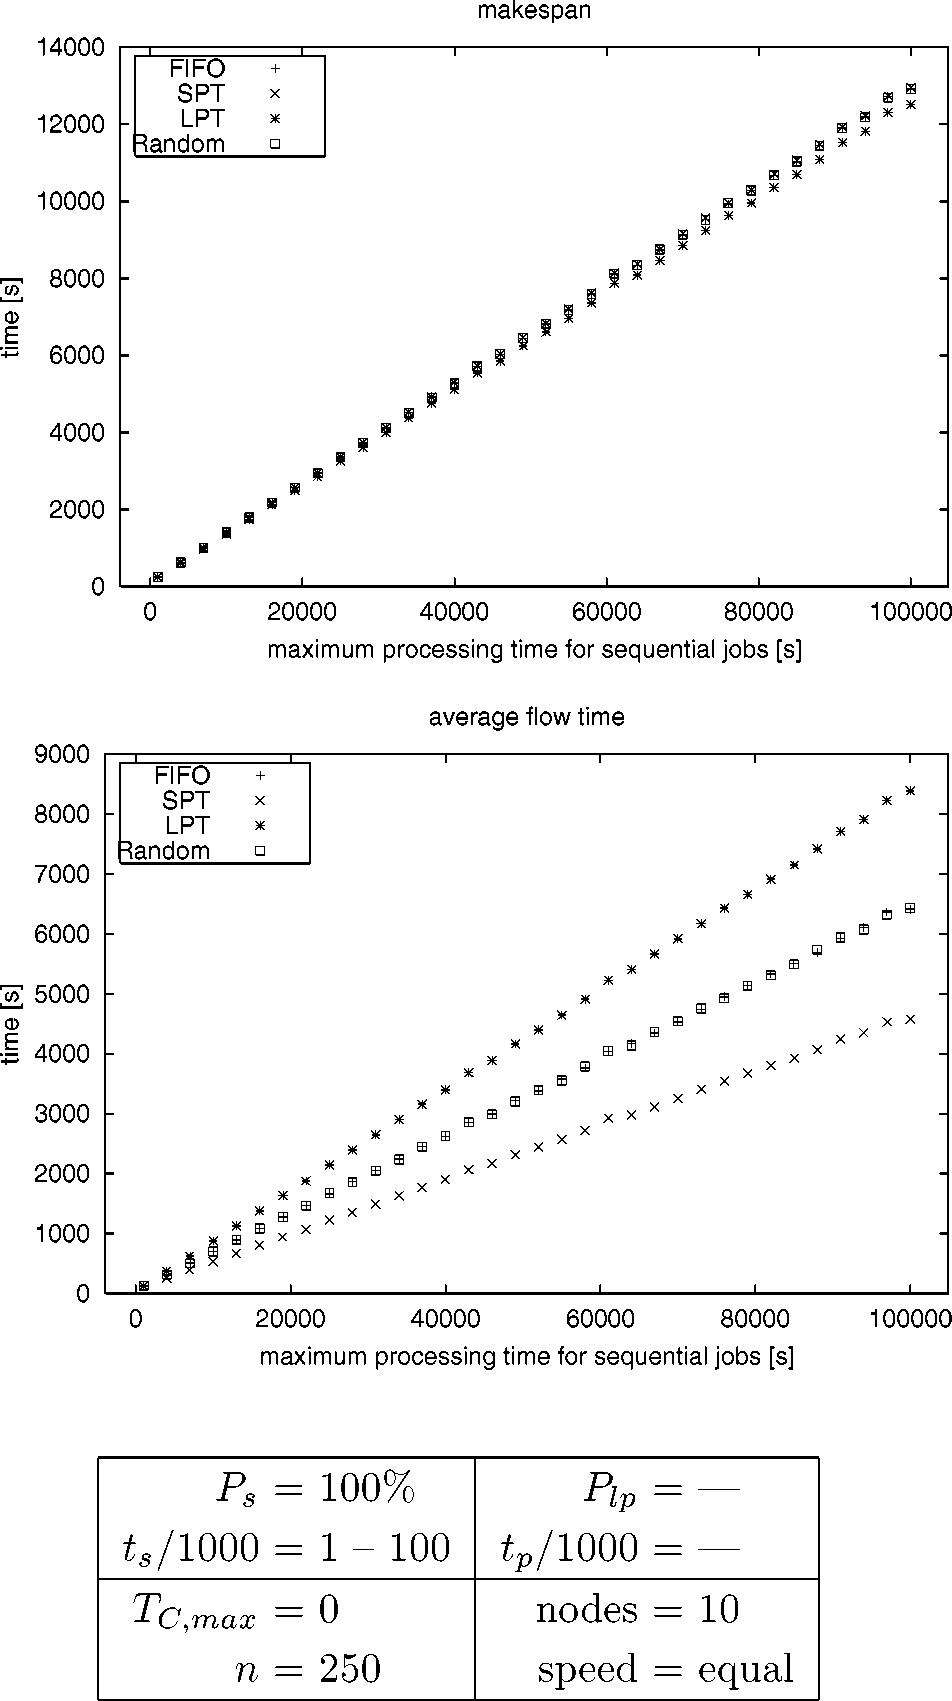
\includegraphics[scale=0.2]{./images/seq0.png}}}
\qquad
\subfloat[label 2]{{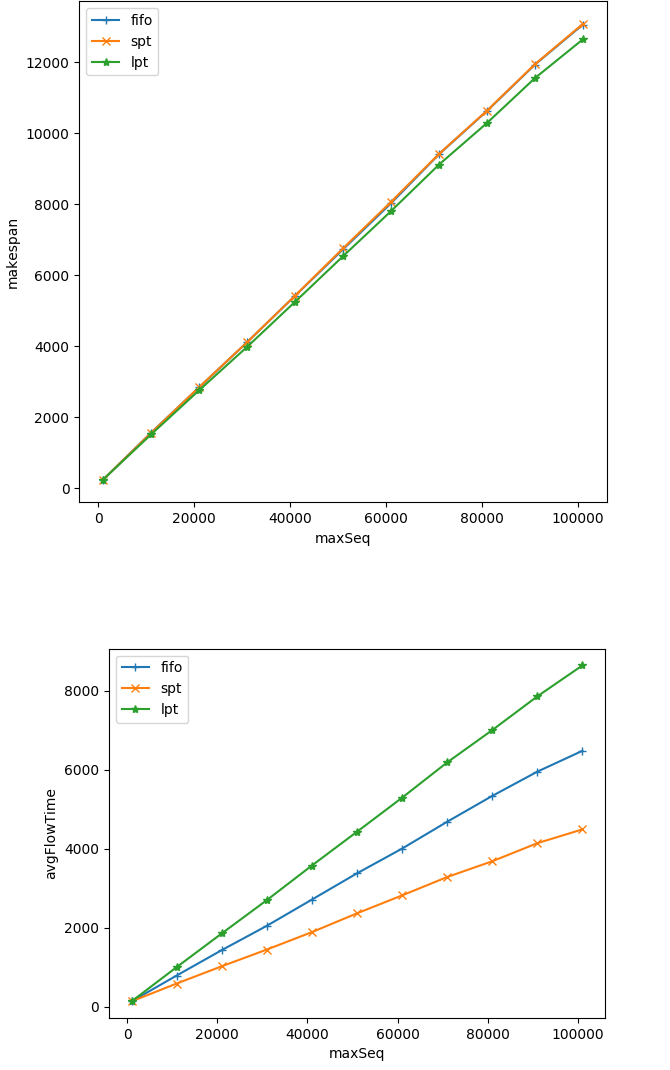
\includegraphics[scale=0.1]{./images/makespan_avgflowtime_seq.png}	
}}	


\end{figure}


\section{Weiterführende Untersuchungen}

\subsection{Backfilling und Fit als Funktionen höherer Ordnung}
\label{chap:higher-order}

Die in Kapitel 2 vorgestellten Funktionen FirstFit und Backfilling sind nur Abwandelungen der FiFo Funktion. Beide wählen den nächsten Auftrag abhängig vom Einreihungszeitpunkt $q_j$, jedoch unter Einschränkungen. "FiFo-Fit" wählt den ersten unter den startbaren Aufträgen aus, "FiFo-BackFilling" wählt den ersten Auftrag, oder einen, der den Bearbeitungsbeginn des ersten Auftrags nicht verzögert. "-Fit" und "-Backfilling" fügen also einen relevanten Kontext hinzu. Es liegt nahe, diese Erweiterungen als Funktionen höherer Ordnung zu betrachten. Ihre Domäne besteht aus einer Scheduling Funktion, den wartenden Aufträgen und einen Kontext - Anzahl an verfügbaren Knoten oder die Abschlusszeitpunkte und die Parallelität der laufenden Aufträge -, und bilden diese partiell auf einen Auftrag ab. 
Da FirstFit-Backfilling von [PaperZitat] als Sieger auserkohren wurde, LPT und GPT aber nicht im Backfilling Kontext untersucht wurden, wird im folgenden untersucht, ob LPT oder GPT mit -FirstFit oder -Backfilling ähnlich gute Ergebnisse erzielen können.

\paragraph{GPT}
lorem Ipsum

\paragraph{LPT}
lorem Isumpdsfdsakfj



\subsection{Property Based Testing zum Erkenntnisgewinn}
\label{proptest}
\paragraph{Testen statt Simullieren}
Während das Simullieren des Rechenclusters gute Auskunft darüber gibt, wie sich das System bei einer langen Reihe an Aufträgen verhällt, kristalliesiert sich dabei lediglich das durchschnittliche Verhalten heraus. Obwohl diese Analyse sinnvoll ist, um verschiedene Scheduling Funktionen asymptotisch mit einander zu vergleichen, wird durch das Mitteln von hunderten von Läufen nicht ersichtlich, in welchen Fällen eine normalerweise unterlegene Scheduling Funktion einer Anderen überlegen ist.\\
Um eine Intuition für die Unterschiede zwischen Scheduling Funktionen entwickeln zu können ist es hilfreicher, die durch kleinstmögliche Listen an Aufgaben erzeugten Läufe zu vergleichen. Um diese minimalen Beispiele zu generieren, kann ein Property Based Testing Framework verwendet werden. Ein guter Einstiegspunkt in dieses Thema ist [initial Paper 1999]. Hier nur eine kleine Zusammenfassung der für uns wichtigen Aspekte. \\
Ein Test besteht aus einer zu testenden Funktion, eine Eigenschaft, die die Ausgabe der Funktion haben soll, und einem Generator, der Eingaben produziert. Sobald eine Eingabe gefunden wird, deren Ausgabe die geforderte Eigenschaft nicht erfüllt, wird die Eingabe automatisch geschrumptf. Dies führt zu einem leichter interpretierbaren Beispiel, da der ausgegebene Fall "kein Rauschen" enthällt.
Eine Zahl wird geschrumpt, in dem sie verringer wird, ein Tupel von Zahlen, in dem eines der Elemente geschrumpft wird, und eine Liste, in dem Elemnter der Liste weggelassen oder geschrumpft werden.\\
Um ein minimales Beispiel zu finden, in dem Scheduling Funktion $S_1$ Ziel Funktion $T$ besser minimiert als Scheduler $S_2$, können wir die Eigenschaft $T(S_1(x)) >= T (S_2(1))$, mit einem Auftragsgenerator$X$: $(Anzahl Konten,[(\pi_j <= Anzahl Knoten,p_j,q_j)])$ überprüfen.
Ein vom Testframework gefundenes minimales Gegenbeispiel, zeigt uns einen Speziellen Fall, in dem $S_1$ ein besseres Ergebnis erzielt als $S_2$
Für die meinsten Scheduling Funktionen ist das minimal Beispiel eines mit 3 Aufträgen, und einer kleinen Anzahl an Knoten [genaues nochmal testen].

Hier nun einige Beispiele.

\paragraph{Optimistisches Backfilling}
Das vorgestellte "-Backfilling" verfahren wirkt auf den ersten Blick zurückhaltend. Das angegebene Ziel, die zum "-Fit" verglichene Wartezeit gering zuhalten, wird erfüllt, in dem große Aufträge nicht benachteiligt werden. Kleine werden nur vorgezogen, wenn sich dadurch die Wartezeit des besten, aber nicht startbaren Kandidaten nicht verzögert. Dies wird erreicht, in dem ein Auftrag $P'$ nur starten darf, wenn er abgeschlossen wird, bevor der beste Kandidat $P$ startet. Warum aber darf ein Auftrag $P'$, der wenige Knoten benötigt, nicht starten, vorausgesetzt, er nimmt nur so wenige Knoten in anspruch, dass $P$ wie geplant starten kann ($P$ benötigt noch $n$ Knoten zum starten, sobald er starten wird, sind aber $n+k, k>0$ Knoten frei, $\pi_{P'} <= k$).\\
Es ist intuitiv, des es einen Haken gibt, ohne in Scheduling Theorie geübt zu sein, ist es aber nicht einfach, aus dem Stand ein Beispiel zu konstruieren, in dem sich das optimistische -Backfilling negativ auf die Wartezeit auswirkt. Allerdings kann dank Property Based Testing ohne viel Mühe eines generiert werden.
\\(Bild einfügen)
\\Wie in der Grafik erkenn bar, benachteiligt ein solcher optimistisch gestarteter langer, kleiner Auftrag nicht den besten Kandidaten $P_1$, allerdings den zweitbesten Kandidaten $P_2$. Ob dies ein seltener Fall ist, oder ob sich Optimismus im Mittel ausfällt, kann wiederum durch eine Statistische Asuwertung untersucht werden.
\\(vergleichendes Bild einfügen)

\subsection{Simulation von Fehlerhaftem Verhalten}
\label{simErrors}

\paragraph{Lorem}
ipsum